% !TEX root = ../ITGO.tex

%\subsection*{Speed reducer design problem}

In this problem, the total weight of the speed reducer (Figure \ref{fig:SR}) is to be minimized. The problem has seven design variables: face width ($b$), teeth module ($m$), number of teeth on the pinion ($z$), first and second length of shafts between bearings ($l_1$ and $l_2$) and first and second shafts diameter ($d_1$ and $d_2$) \citep{SR}. The problem has 11 nonlinear constraints, and the third variable is constrained to be an integer. A second version of the problem is also found in literature, where the only difference is in the lower bound of the fifth variable (7.8 for SR1 and 7.3 for SR2). The objective function value at the optimal is $f(\bm{x}^*) = 2996.34816497$ for the first version (SR1), and $f(\bm{x}^*) = 2994.471066$ for the second version (SR2). The mathematical formulation of the problem follows:

\vspace{-0.5cm}

\begin{align*}
\textbf{Minimize:} & \\
& f(\bm{x}) = 0.7854x_1x_2^2(3.333x_3^2 + 14.9334x_3 - 43.0934) \\
& \quad \qquad - 1.508x_1(x_6^2 + x_7^2) + 7.4777(x_6^3 + x_7^3) \\
& \quad \qquad + 0.7854(x_4 x_6^2 + x_5x_7^2) \\[0.5em]
\textbf{subject to:} &\\
& g_1(\bm{x}) = \frac{27}{x_1x_2^2x_3} - 1 \leq 0 \\
& g_2(\bm{x}) = \frac{397.5}{x_1x_2x_3^2} - 1 \leq 0 \\
& g_3(\bm{x}) = \frac{1.93x_4^3}{x_2x_3x_6^4} -1 \leq 0 \\
& g_4(\bm{x}) = \frac{1.93x_5^3}{x_2x_3x_7^4} -1 \leq 0 \\
& g_5(\bm{x}) = \frac{1}{110x_6^3} \sqrt{\Big( \frac{745x_4}{x_2x_3} \Big)^2 + 16.9 \times 10^6} - 1 \leq 0 \\
& g_6(\bm{x}) = \frac{1}{85x_7^3} \sqrt{\Big( \frac{745x_5}{x_2x_3} \Big)^2 + 157.5 \times 10^6} - 1 \leq 0 \\
& g_7(\bm{x}) = \frac{x_2x_3}{40} - 1 \leq 0 \\
& g_8(\bm{x}) = \frac{5x_2}{x_1} - 1 \leq 0 \\
& g_9(\bm{x}) = \frac{x_1}{12x_2} - 1 \leq 0 \\
& g_{10}(\bm{x}) = \frac{1.5x_6 + 1.9}{x_4} - 1 \leq 0 \\
& g_{11}(\bm{x}) = \frac{1.1x_7 + 1.9}{x_5} - 1 \leq 0 \\[0.5em]
\textbf{with bounds:} & \\
& 2.6 \leq x_1 \leq 3.6, \quad 0.7 \leq x_2 \leq 0.8, \quad 17 \leq x_3 \leq 28, \quad x_3 \in \mathbb{Z} \\
& 7.3 \leq x_4 \leq 8.3, \quad 7.8 \leq x_5 \leq 8.3 \ (\text{or} \ 7.3 \leq x_5 \leq 8.3) \\
& 2.9 \leq x_6 \leq 3.9, \quad 5.0 \leq x_7 \leq 5.5
\end{align*}

\vspace{0.5cm}

\begin{figure}[h]
    \begin{center}
    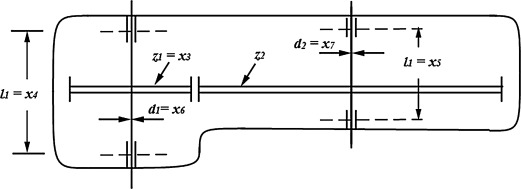
\includegraphics[scale=0.6]{img/Problems/SR.jpg}
    \end{center}
    \captionsetup{justification=centering}
    \caption{Schematic view of the speed reducer design problem.}\label{fig:SR}
\end{figure}
